% !TEX root = slides.tex

\documentclass[
    %draft, % enable for quick rendering
    9pt,aspectratio=169,usepdftitle=false,
    %handout, % enable for uncover suppression
    hyperref={breaklinks},
    xcolor={svgnames}]{beamer}

% Load used-defined config
% !TEX root = slides.tex

\usepackage{expl3}
\usepackage{xparse}

%%%%%%%%%%%%
% Metadata %
%%%%%%%%%%%%

\ExplSyntaxOn

\tl_new:N   \l__configsupport_title_tl
\tl_new:N   \l__configsupport_author_tl
\tl_new:N   \l__configsupport_iso_date_tl
\tl_new:N   \l__configsupport_faculty_tl
\tl_new:N   \l__configsupport_chair_tl
\tl_new:N   \l__configsupport_workgroup_tl
\bool_new:N \l__configsupport_english_bool

\ProvideExpandableDocumentCommand{\settalktitle}{m}{
    \tl_set:Nn \l__configsupport_title_tl {#1}
}
\ProvideExpandableDocumentCommand{\talktitle}{}{\tl_use:N \l__configsupport_title_tl}

\ProvideExpandableDocumentCommand{\settalkauthor}{m}{
    \tl_set:Nn \l__configsupport_author_tl {#1}
}
\ProvideExpandableDocumentCommand{\addtalkauthor}{m}{
    \tl_if_empty:NF \l__configsupport_author_tl { \tl_put_right:Nn \l__configsupport_author_tl {,\ } }
    \tl_put_right:Nn \l__configsupport_author_tl {#1}
}
\ProvideExpandableDocumentCommand{\talkauthor}{}{\tl_use:N \l__configsupport_author_tl}

\ProvideExpandableDocumentCommand{\settalkisodate}{m}{
    \tl_set:Nn \l__configsupport_iso_date_tl {#1}
}
\ProvideExpandableDocumentCommand{\talkisodate}{}{\tl_use:N \l__configsupport_iso_date_tl}
\ProvideExpandableDocumentCommand{\talkdate}{}{\exp_args:Nf \DTMDate \talkisodate}

\ProvideExpandableDocumentCommand{\setfaculty}{m}{
    \tl_set:Nn \l__configsupport_faculty_tl {#1}
}
\ProvideExpandableDocumentCommand{\faculty}{}{\tl_use:N \l__configsupport_faculty_tl}

\ProvideExpandableDocumentCommand{\setchair}{m}{
    \tl_set:Nn \l__configsupport_chair_tl {#1}
}
\ProvideExpandableDocumentCommand{\chair}{}{\tl_use:N \l__configsupport_chair_tl}

\ProvideExpandableDocumentCommand{\setworkgroup}{m}{
    \tl_set:Nn \l__configsupport_workgroup_tl {#1}
}
\ProvideExpandableDocumentCommand{\workgroup}{}{\tl_use:N \l__configsupport_workgroup_tl}

\ProvideExpandableDocumentCommand{\germantalk}{}{
    \bool_set_false:N \l__configsupport_english_bool
}

\ProvideExpandableDocumentCommand{\englishtalk}{}{
    \bool_set_true:N \l__configsupport_english_bool
}

\ProvideExpandableDocumentCommand{\languagesetup}{}{
    \bool_if:NTF \l__configsupport_english_bool {
        \setdefaultlanguage[variant=usmax]{english}
        \setotherlanguage[variant=german, latesthyphen=true]{german}
    } {
        \setdefaultlanguage[variant=german, latesthyphen=true]{german}
        \setotherlanguage[variant=usmax]{english}
    }
}

\ExplSyntaxOff

%%%%%%%%%%%%%%%%%%%%%%
% Shorthand commands %
%%%%%%%%%%%%%%%%%%%%%%

\ProvideExpandableDocumentCommand{\aquaheader}{}{
    \setfaculty{Fakultät für Informatik}
    \setchair{Lehrstuhl 14 für Software Engineering}
    \setworkgroup{Arbeitsgruppe AQUA}
}
% !TEX root = slides.tex

%%%%%%%%%%%%%%%%%%
% Metadata setup %
%%%%%%%%%%%%%%%%%%

% Talk's title
\settalktitle{Meta Programming System: An Introduction}

% Author's name
\settalkauthor{Till Schallau}
% Multiple authors' names
% \addtalkauthor{John Doe}

% Talk date (ISO date format)
\settalkisodate{2020-09-28}

% Header metadata
\aquaheader

%%%%%%%%%%%%%%%%%%%%%%
% Language selection %
%%%%%%%%%%%%%%%%%%%%%%

%\germantalk
\englishtalk

%%%%%%%%%%%%
% Packages %
%%%%%%%%%%%%

% Should go first:

% Font control
\usepackage{fontspec}

% Math support
\usepackage{amsmath}
\usepackage{unicode-math}

% Font selection (needs to go before polyglossia)
\usepackage{libertinus}

% Language control
\usepackage{polyglossia}
\languagesetup

% Date formats
\usepackage[useregional]{datetime2}

% Algorithms
\usepackage[linesnumbered, vlined]{algorithm2e}

% Author and title reuse
\usepackage{authoraftertitle}

% Bibliography
\usepackage[style=alphabetic]{biblatex}

% Print-quality tables
\usepackage{booktabs}

% Watermarks for draft versions
%\usepackage{draftwatermark}
%\SetWatermarkAngle{57.5}
%\SetWatermarkLightness{.95}
%\SetWatermarkText{ENTWURF \(\alpha\).1}

% Image inclusion
\usepackage{graphicx}

% Enable microtypography support
\usepackage[final]{microtype}

% Listings with syntax highlighting; requires --shell-escape
\usepackage[newfloat]{minted}

% Fine spacing control for math
\usepackage{mleftright}

% PDF inclusion
\usepackage{pdfpages}

% Relative font sizes
\usepackage{relsize}

% URL's
\usepackage{url}

\usepackage[os=win]{menukeys}

% Drawings and Graphs
\usepackage{tikz}
\usetikzlibrary{babel}
\usetikzlibrary{calc}
\usetikzlibrary{external} % requires --shell-escape
\usetikzlibrary{positioning}
\tikzsetexternalprefix{tikz-externals}
% \tikzexternalize Render TikZ externally, fails for some references
\usepackage{pgfplots}
\pgfplotsset{compat=1.17}

% Needs to go last:

% Language-sensitive quotation marks
\usepackage{csquotes}

% Break URLs at / and -
\def\UrlBreaks{\do\/\do-}

%%%%%%%%%%%%%%%%%%%%
% Style and layout %
%%%%%%%%%%%%%%%%%%%%

% Load Theme
\usetheme{TUDo}
\titlegraphic{illustrations/Spektralringe}

% Neat + for et al
\renewcommand*{\labelalphaothers}{\raisebox{.3ex}{\relsize{-3}{\bfseries +}}}
\renewcommand*{\sortalphaothers}{+}

% Remove algorithm captions, see examples
\renewcommand{\AlCapSty}{}

% Use minted's line numbers for algorithm2e
\let\vrbstyle\theFancyVerbLine
\patchcmd{\vrbstyle}{\arabic{FancyVerbLine}}{}{}{}
\SetNlSty{vrbstyle}{}{}

% Pastel colored listings
\usemintedstyle{friendly}

% German strings
\addto\captionsgerman{%
    \renewcommand{\listlistingname}{Listingverzeichnis}%
}

%%%%%%%%%%%
% Content %
%%%%%%%%%%%

% Load external resources
\addbibresource{bibliography.bib}

% Internal metadata setup
\title{\talktitle}
\author{\talkauthor}
\date{\talkdate}

\institute{%
    \faculty

    \chair

    \workgroup%
}

\AtBeginSection[]{
    \begin{frame}<beamer>
        \frametitle{\contentsname}
        \tableofcontents[
            currentsection,
            currentsubsection,
            hideothersubsections,
            sectionstyle=show/shaded,
        ]
    \end{frame}
}

 \newcommand{\workshoplanguage}[1]{
\includegraphics[height=6px]{graphics/language.png} de.tudo.cs.ls14.aqua.mps.workshop.#1}

\newcommand{\workshoplanguagecreation}[0]{
\includegraphics[height=6px]{graphics/language.png} Language}
\newcommand{\workshopsolution}[1]{
\includegraphics[height=6px]{graphics/solution.png} de.tudo.cs.ls14.aqua.mps.workshop.#1}
\newcommand{\workshopmodel}[1]{
\includegraphics[height=6px]{graphics/model.png} #1}
\newcommand{\workshopnode}[1]{
\includegraphics[height=6px]{graphics/node.png} #1}
\newcommand{\workshopproject}[0]{
\includegraphics[height=6px]{graphics/project.png} mps-workshop}
\newcommand{\workshoprun}[0]{
\includegraphics[height=6px]{graphics/run.png} Run 'Node de.tudo.cs.ls14...'}
\newcommand{\workshopmoduleproperties}[0]{
\includegraphics[height=6px]{graphics/properties.png} Module Properties}
\newcommand{\workshopruntime}[0]{
\includegraphics[height=6px]{graphics/runtime.png} Runtime}
\newcommand{\workshopversion}[0]{\menu{
\includegraphics[height=6px]{graphics/version.png} Get from Version Control}}
\newcommand{\workshopinspector}[0]{
\includegraphics[height=6px]{graphics/inspector.png} Inspector}
\newcommand{\workshopintention}[0]{
\includegraphics[height=6px]{graphics/intention.png} Intention}
\newcommand{\workshopconfiguration}[0]{
\includegraphics[height=6px]{graphics/configuration.png} Mapping Configuration}
\newcommand{\workshoptemplate}[0]{
\includegraphics[height=6px]{graphics/template.png} Template}
\newcommand{\workshoptextgen}[0]{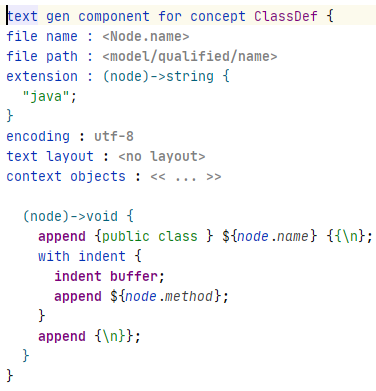
\includegraphics[height=6px]{graphics/textgen.png} TextGen}
